%\subsection{Effect of Attention Width}
Our model has a parameter $K$ that specifies the number of entities to attend to. To illustrate
the effect of $K$, we evaluated performance on the testa Conll datasets, for several values of $K$. Results 
are shown in \figref{fig:k_effect}. It can be seen that performance peaks at $K=3$, with a sharp decrease after $K=10$. 

\begin{figure}
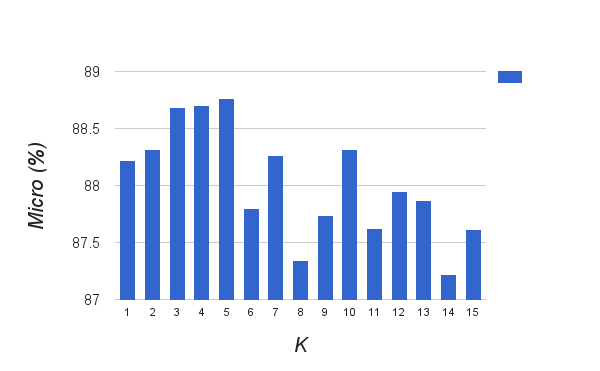
\includegraphics[width=\linewidth]{./k_effect.png}
\caption{Effect of parameter $K$ on entity linking accuracy. Results shown for the testa Conll dataset, where the model
is trained on Conll training data. }
\label{fig:k_effect}
\end{figure}